\scanpage{50}
\mspage{\handwritten{6}}

\begingroup
\setbox0=\vbox{%
  \small
  \hsize=\linewidth
  \parindent=0pt
  \parskip=.45\baselineskip
  Pour la première assertion, on se ramène encore, par descente et en utilisant \deleted{1}\handwritten{4}.\handwritten{3}, au cas où $k$ est séparablement clos. Procédant comme dans la démonstration de \deleted{1}\handwritten{4}.6 , on déduit de \deleted{1}\handwritten{4}.5 et de l'hypothèse sur $L$ que $\underline{L}$ \deleted{provient} est isomorphe à l'image inverse d'un Module birigidifié $\underline{M}$ sur $A\mathbin{\mathrm{x}}Q$, et pour la première assertion de \deleted{1}\handwritten{4}.7, on est donc ramené au cas $A=P$. Or $\underline L$ définit un morphisme de schémas ponctués
  \[
    f\colon Q\handwritten{\longrightarrow}\underline{\mathrm{P}\deleted{\unsure{j|i}}\mathrm{ic}}_{P/k}\ ,
  \]
  qui se factorise nécessairement par le schéma abélien dual $P'$ de $P$. Soit $\underline{L}'$ l'image inverse du faisceau de Weil sur $P\mathbin{\mathrm{x}}P'$ par \deleted{$\mathrm{id}_{P}\mathbin{\mathrm{x}}\mathrm{id}$}
  \[
    \deleted{p}\mathrm{id}_{P}\mathbin{\mathrm{x}}f\colon P\mathbin{\mathrm{x}}Q\handwritten{\longrightarrow}P\mathbin{\mathrm{x}}P'\ ,
  \]
  c'est un Module birigidifié qui, par définition de $f$, ne diffère \deleted{q}de $\underline L$ que modulo l'image inverse d'un Module inversible $\underline M$ sur $P$. Comme $\underline L'$ et $\underline L$ ont une restriction triviale à $\deleted{\unsure{e|E}}P\mathbin{\mathrm{x}}e_{Q}$ , on en conclut que $\underline M$ est triv\unsure{\deleted{a}i\deleted{i}a|\deleted{i}a\deleted{a}i}l, donc que $\underline L$ est isomorphe à $\underline L'$. Or nous avons signalé dans VII 2.9.4 \deleted{p}que sur un produit de deux schémas abéliens, les correspondances divisorielles provenaient de biextensions. Il en résulte que $\underline L'$ , \deleted{\unsure{et en|et ea}} ou \unsure{\deleted{p}c|p}e qui revient au même, $\underline L$ , provient d'une biextension.\par

  Revenant au cas généfal ($P$ extension de $A$ par $L$), \unsure{\deleted{e}i\deleted{t}l|\deleted{i}e\deleted{l}t} reste à prouver que (\deleted{1}\handwritten{4}.7.1) est bien un isomorphisme. Mais cela résulte de la suite exacte des $\mathrm{B}\rlap{\begin{tikzpicture}[overlay,baseline=0pt,x=1em,y=1ex,line cap=round]
    \draw[line width=.5pt] (.02,-.35) -- (.23,-.35) -- (.27,-.7);
  \end{tikzpicture}}\bar{\mathrm{i}}\mathrm{ext}^{i}$ ($i=0,1$) associée à la suite exacte
  \[
    0\rlap{\begin{tikzpicture}[overlay,baseline=0pt,x=1em,y=1ex,line cap=round]
      \draw[line width=.55pt] (.45,.35) .. controls (.12,-.1) and (.22,-.65) .. (.65,-1.4);
    \end{tikzpicture}}\handwritten{\longrightarrow}L\handwritten{\longrightarrow}P\handwritten{\longrightarrow}A\handwritten{\longrightarrow}0\ ,
  \]
  et des relations
  \[
    \operatorname{Biext}^{o}(L,Q;\underline G_{m})=0\ ,\quad
    \operatorname{Biext}^{1}(L\overset{\unsure{\mathrm{x}|\deleted{\mathrm{x}}}}{,}Q;\underline G_{m})=0\ ,
  \]
  dont la premièr\unsure{\deleted{u}e|ë} est un cas parti\unsure{\deleted{v}c|\deleted{c}v}ulier de l'assertion de rigidité faite dans \deleted{1}\handwritten{4}.\handwritten{3} , et la deuxième n'est autre que le premier cas de \deleted{1}\handwritten{4}.6.\par

  \setbox2=\vbox{%
    \hsize=\linewidth
    \parindent=0pt
    \uline{Corollaire} \deleted{1}\handwritten{4}.8. Sous les conditions de \deleted{1}\handwritten{4}.7, supposons que $Q$ soit extension d'un groupe algébrique $B$ (néces\unsure{\inserted{s}a|\deleted{s}a}irement lisse et connexe) par un\par
  }%
  \edef\corollaryheight{\the\ht2}
  \noindent\hbox{%
    \rlap{\begin{tikzpicture}[overlay,baseline=0pt,x=1em,y=\corollaryheight,line cap=round]
      \draw[line width=.65pt] (-.75,1) .. controls (-.84,.93) and (-.81,.6) .. (-.8,.4)
        .. controls (-.78,.2) and (-.72,.08) .. (-.7,0);
      \draw[line width=1.05pt] (-.77,.25) -- (-.7,0);
    \end{tikzpicture}}%
    \box2
  }\par
}%
\edef\scanblockwidth{\the\wd0}
\edef\scanblockheight{\the\ht0}
\noindent\hbox{%
  \rlap{\raise\ht0\hbox{%
    \begin{tikzpicture}[overlay,baseline=0pt,x=\scanblockwidth,y=-\scanblockheight,line cap=round]
      \draw[black!55,line width=.5pt]
        (.125,-.015) .. controls (.12,-.04) and (.15,-.03) .. (.17,.01)
        .. controls (.27,.17) and (.60,.65) .. (.746,.98);
      \draw[black!28,line width=.45pt]
        (.516,.018) .. controls (.56,.095) and (.73,.37) .. (.849,.564);
      \draw[black!45,line width=.5pt]
        (.059,.516) .. controls (.10,.523) and (.12,.55) .. (.136,.59)
        .. controls (.22,.74) and (.31,.86) .. (.372,.917);
    \end{tikzpicture}%
  }}%
  \box0
}\par
\endgroup

% archive sheet number: 49
